\documentclass[a4paper]{tufte-handout}

\usepackage{/Users/paulallen/OU/Maths/style}

\begin{document}
\tma{00}

\begin{question}
\bigskip
\[x= \frac{-b\pm\sqrt{(b^{2}-4ac)}}{2a}\]
\end{question}

\begin{question}
\bigskip
\[xy \times xz = x^{2}yz\]
\end{question}

\begin{question}
\bigskip

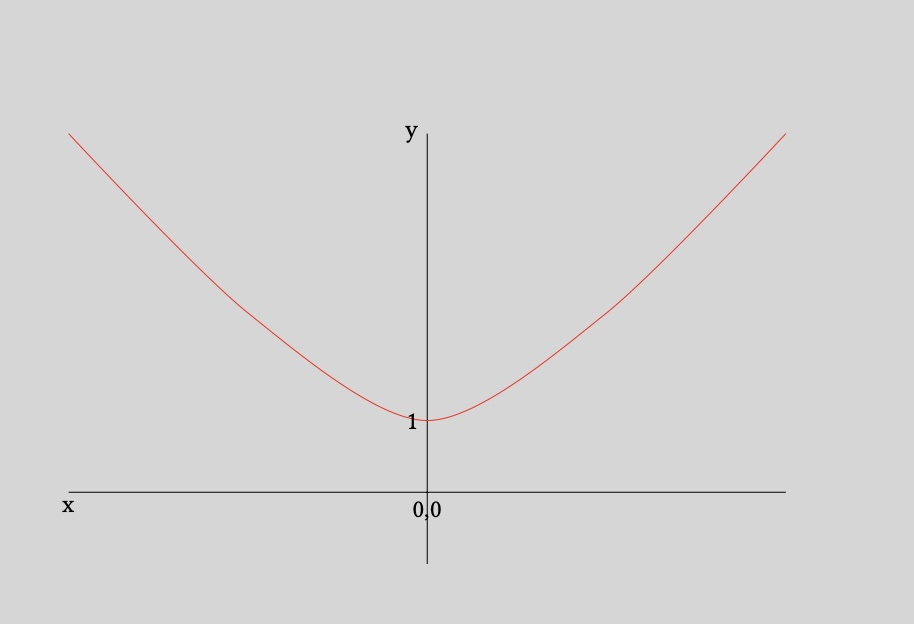
\includegraphics{Graph.jpg}
\end{question}

\begin{question}

\bigskip
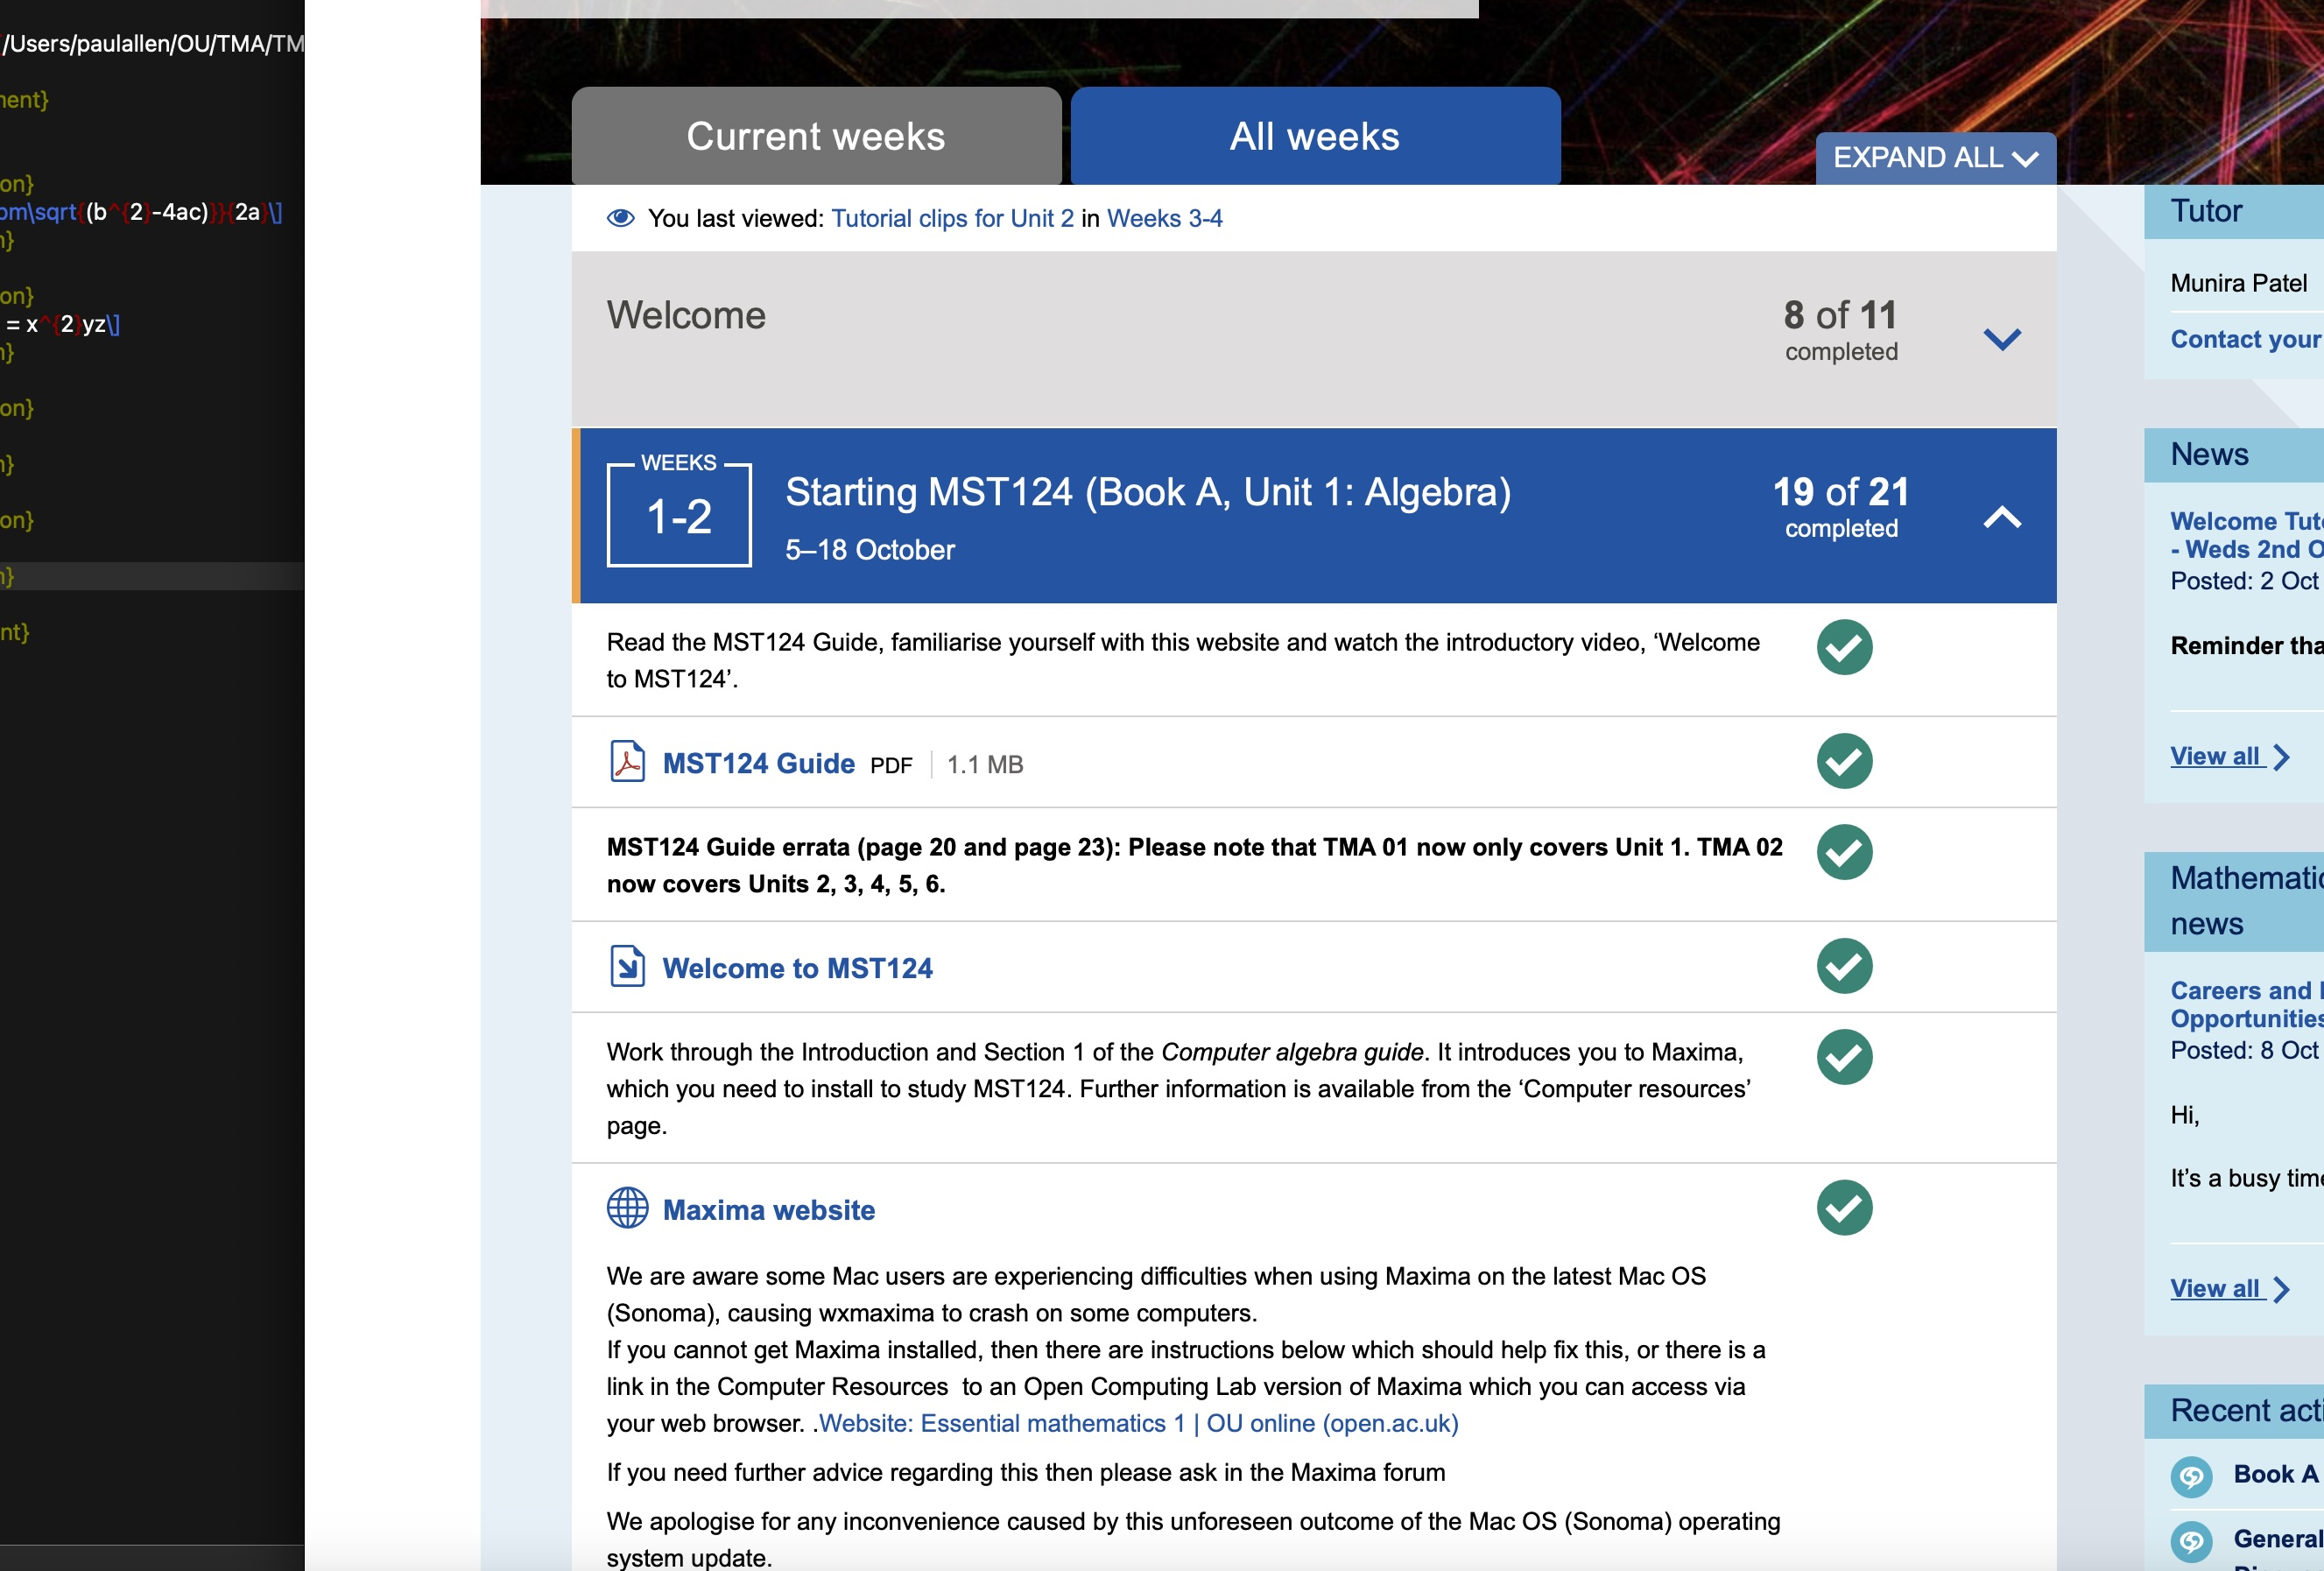
\includegraphics[scale=0.3]{screen_shot_TMA00.jpg}
\end{question}

\begin{question}
Solve the equation:

\[\frac{x}{5} - (1 + x) = \frac{2}{3}\]

\hfill{Eliminate fractions by multiplying by the LCM, 15.}
\[
15 \left[\frac{x}{5} - (1 + x)\right] = 15 \cdot \frac{2}{3}
\]

\hfill{Distribute the \(15\).}
\[
\frac{15x}{5} - 15(1 + x) = \frac{30}{3}
\]

\hfill{Simplify.}
\[
3x - 15 - 15x = 10
\]

\hfill{Combine like terms.}
\[
-12x - 15 = 10
\]

\hfill{Add \(15\) to both sides to isolate \(x\).}
\[
-12x = 25
\]

\hfill{Divide by \(-12\) to solve for \(x\).}
\[
x = \frac{-25}{12}
\]

\end{question}

\end{document}